\sectionwithlogo{Аффинные преобразования}
	{\includeMPgraphics{figure-cat-transformed}}

\begin{frame}{Определение аффинных преобразований плоскости}
\emph{Аффинные преобразования} плоскости задаются шестёркой чисел $\alert<2>{T_{xx}}$,
$\alert<2>{T_{xy}}$, $\alert<2>{T_x}$, $\alert<2>{T_{yx}}$,
$\alert<2>{T_{yy}}$, $\alert<2>{T_y}$ при помощи формул:
{\LARGE
	\[
	\begin{aligned}
	&\alert<3>{x'}=\alert<2>{T_{xx}}\,\alert<4>{x}+\alert<2>{T_{xy}}\,\alert<4>{y}+\alert<2>{T_x}\\
	&\alert<3>{y'}=\alert<2>{T_{yx}}\,\alert<4>{x}+\alert<2>{T_{yy}}\,\alert<4>{y}+\alert<2>{T_y}
	\end{aligned}
	\]
}

\uncover<3->{\alert<3>{Новые} координаты точки выражаются через \alert<4>{старые} линейным образом.}
\transdissolve<2->
\end{frame}

\begin{frame}{Невырожденность аффинных преобразований}
\emph{Невырожденным} называется аффинное преобразование, если
{\LARGE
	\[
	T_{xx}T_{yy}-T_{xy}T_{yx}\ne0.
	\]
}
\end{frame}

\begin{frame}{Свойства невырожденных аффинных преобразований}
\begin{itemize}
\item
прямые преобразуются в~прямые
\item
параллельные прямые преобразуются в~параллельные прямые
\item
вполне определяется тремя точками~— вершинами треугольника, и~тремя их образами
\end{itemize}
\end{frame}

\begin{frame}{Кошки Арнольда}
Академик В.~И.~Арнольд очень любил кошек.

Он придумал иллюстрировать преобразования плоскости при помощи кошачьих морд.
\bigskip
\begin{center}
\only<1->{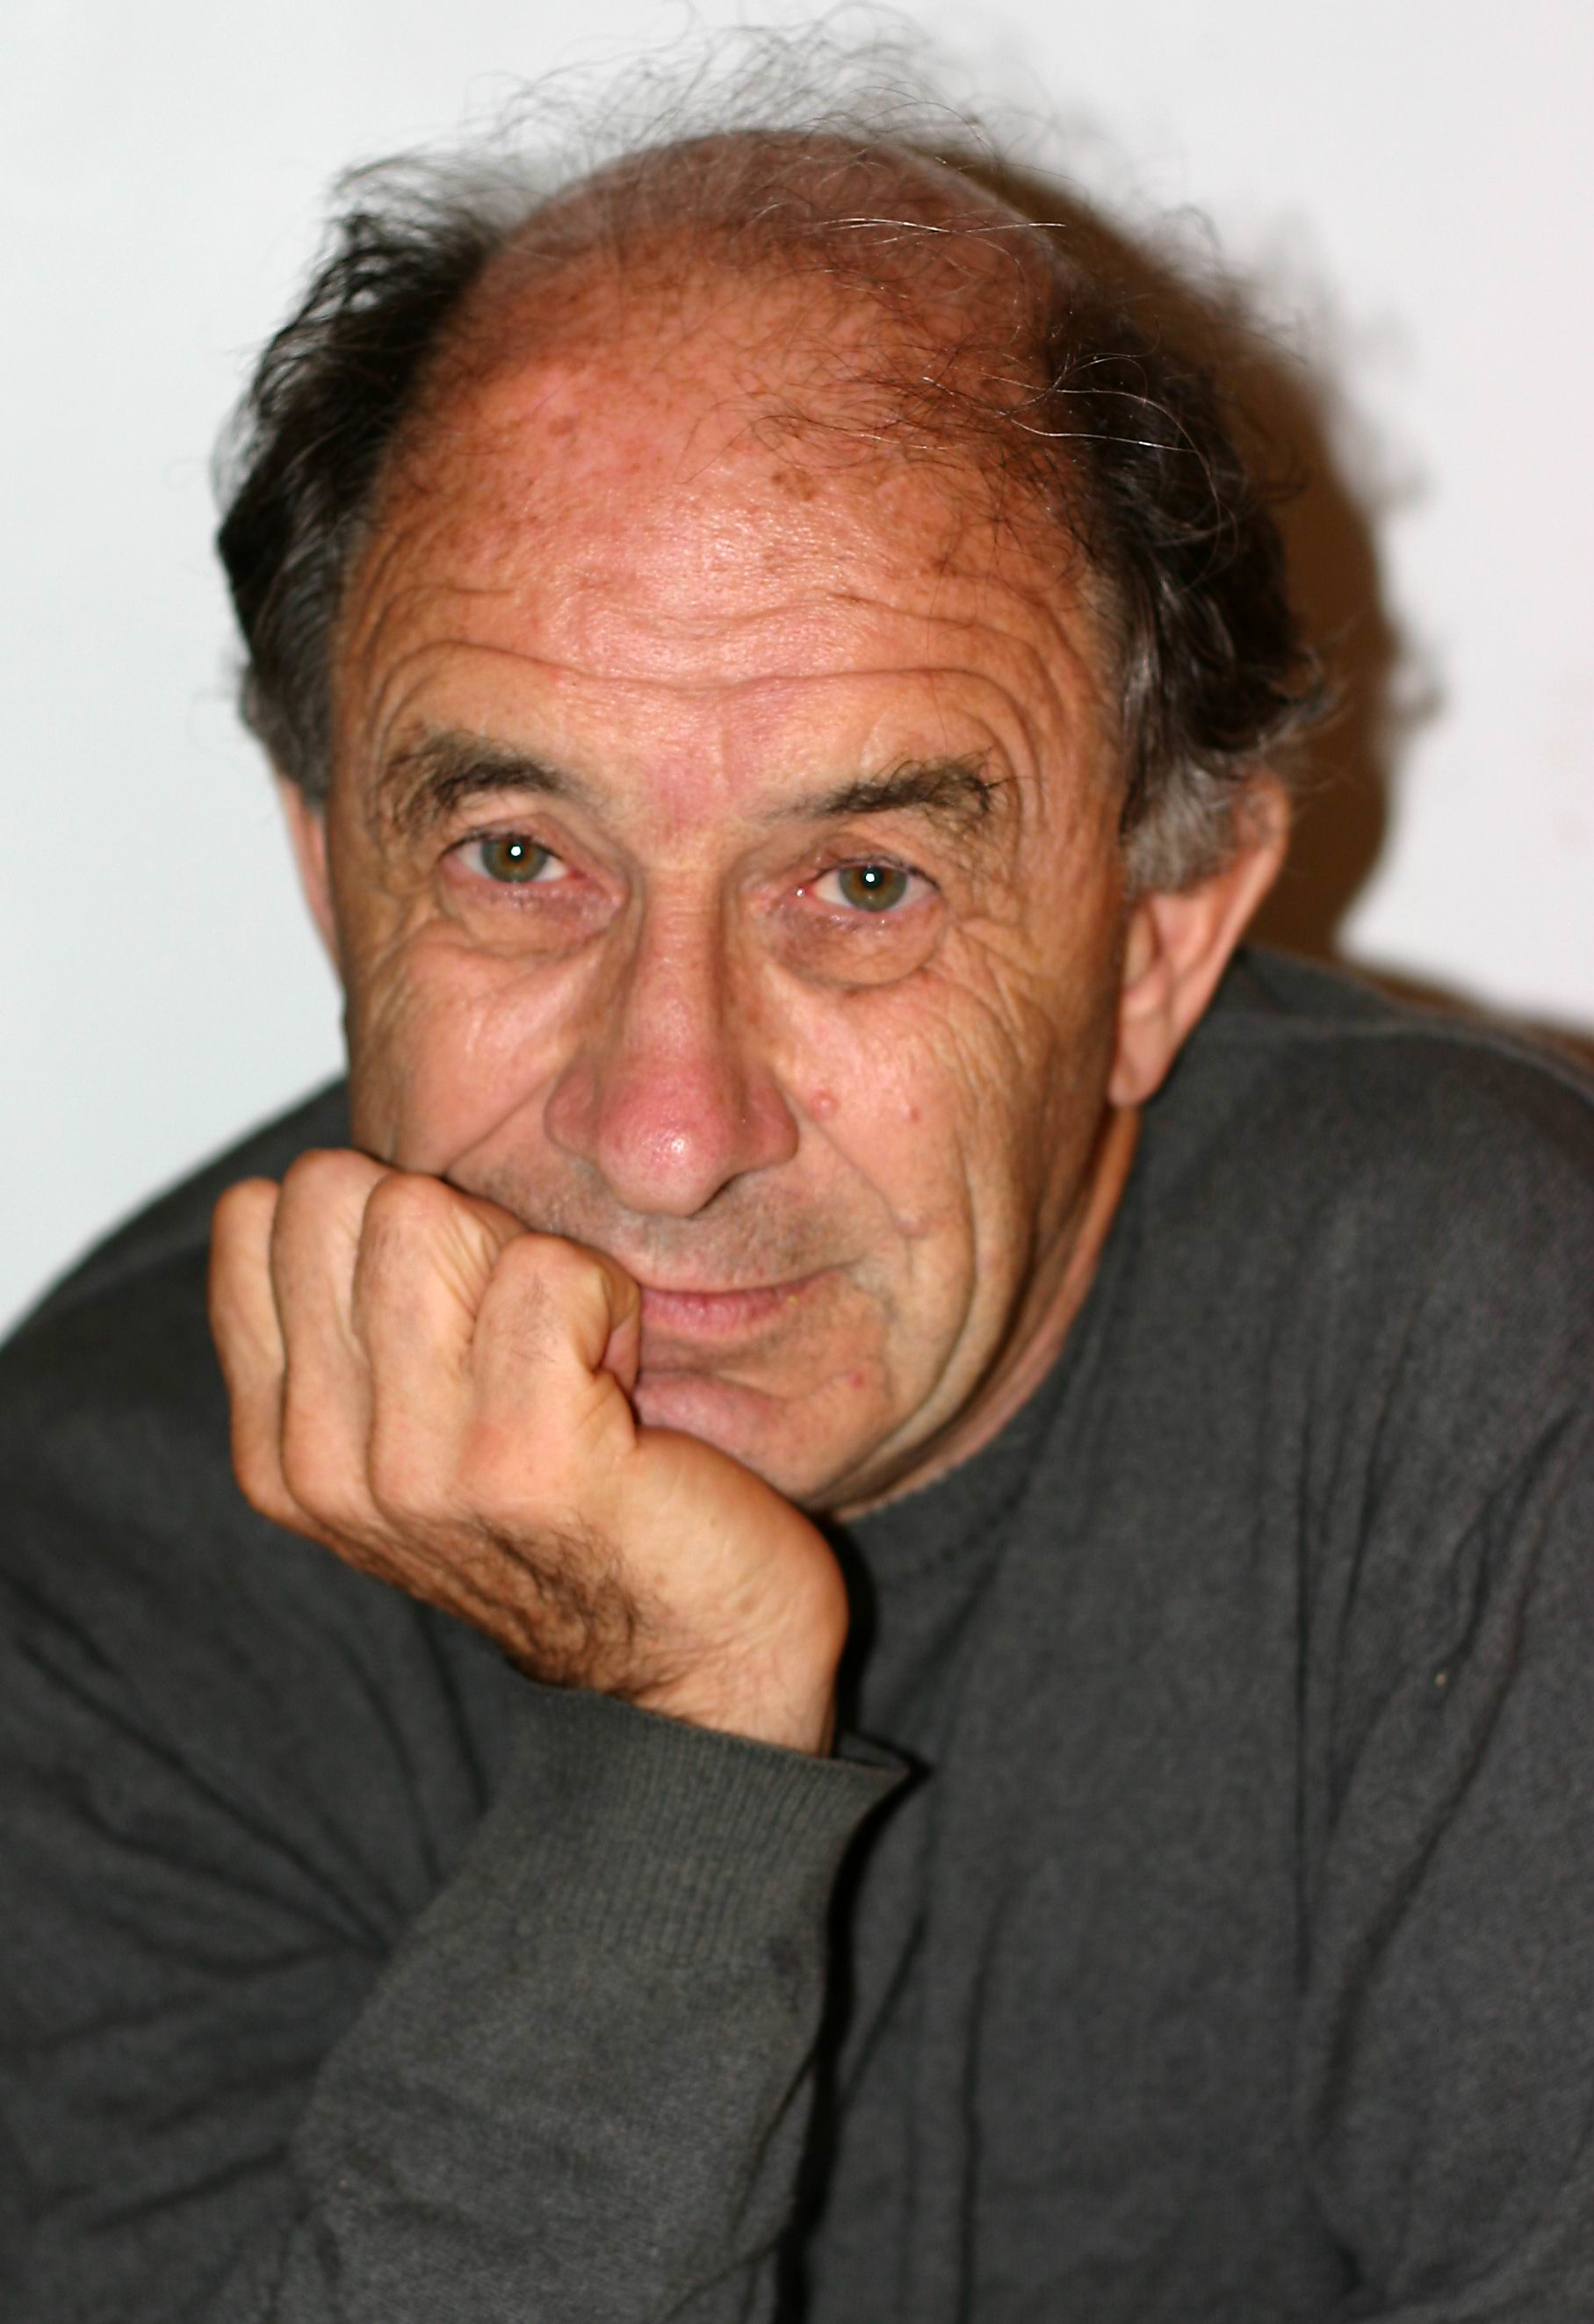
\includegraphics[height=124.874434pt]{figure-arnold}}%
\only<2>{\quad\includeMPgraphics{figure-cat}}%
\end{center}
\end{frame}

\begin{frame}{Тождественное преобразование}
\begin{center}
\LARGE
\includeMPgraphics{figure-cat-identity}\\[4ex]
\literal{identity}%
\end{center}
\end{frame}

\begin{frame}{Сдвиг (параллельный перенос)}
\begin{center}
\LARGE
\only<1>{\includeMPgraphics{figure-cat-shifted}\\[4ex]
\literal{identity shifted (.75, .5)}}%
\only<2>{%
$(x,y)$ \literal{shifted} $(a,b)$\\
$\equiv$\\
$(x+a,y+b)$
}%
\end{center}
\end{frame}

\begin{frame}{Поворот}
\begin{center}
\LARGE
\only<1>{\includeMPgraphics{figure-cat-rotated}\\[4ex]
\literal{identity rotated 60}}%
\only<2>{%
$(x,y)$ \literal{rotated} $\theta$\\
$\equiv$\\
$(x\cos\theta-y\sin\theta,x\sin\theta+y\cos\theta)$
}%
\end{center}
\end{frame}

\begin{frame}{Растяжение}
\begin{center}
\LARGE
\only<1>{\includeMPgraphics{figure-cat-scaled-1}}%
\only<2>{\includeMPgraphics{figure-cat-scaled-2}}%
\only<1,2>{\\[4ex]
\literal{identity scaled \only<1>{1.5}\only<2>{-.5}}}%
\only<3>{%
$(x,y)$ \literal{scaled} $k$\\
$\equiv$\\
$(kx,ky)$
}%
\end{center}
\end{frame}

\begin{frame}{Анаморфотные преобразования}
\begin{center}
\LARGE
\only<1>{\includeMPgraphics{figure-cat-xscaled}}%
\only<3>{\includeMPgraphics{figure-cat-yscaled}}%
\only<1,3>{\\[4ex]
\literal{identity \only<1>{\alert{x}scaled 2.5}\only<3>{\alert{y}scaled .25}}}%
\only<2,4>{%
$(x,y)$ \literal{\only<2>{x}\only<4>{y}scaled} $k$\\
$\equiv$\\
$(\only<2>{k}x,\only<4>{k}y)$
}%
\end{center}
\end{frame}

\begin{frame}{Наклон}
\begin{center}
\LARGE
\only<1>{\includeMPgraphics{figure-cat-slanted}\\[4ex]
\literal{identity slanted 2}}%
\only<2>{%
$(x,y)$ \literal{slanted} $k$\\
$\equiv$\\
$(x+ky,y)$
}%
\end{center}
\end{frame}

\begin{frame}{Поворот вокруг заданной точки}
\begin{center}
\LARGE
\only<1>{\includeMPgraphics{figure-cat-rotatedabout}%
\\[4ex]
\literal{identity}\par
\literal{rotatedabout((1, 1), 90)}}%
\only<2>{%
$p$ \literal{rotatedabout(}$z$\literal{, }$\theta$\literal{)}\\
$\equiv$\\
$p$ \literal{shifted} $-z$ \literal{rotated} $\theta$ \literal{shifted} $z$
}%
\end{center}
\end{frame}

\begin{frame}{Осевая симметрия (зеркальное отражение)}
\begin{center}
\includeMPgraphics{figure-cat-reflectedabout}%
\\[4ex]
{\LARGE
\literal{identity}\par
\literal{reflectedabout((0, .5), (1, 1))}}%
\end{center}
\end{frame}

\begin{frame}{Аффинное преобразование общего вида}
\begin{center}
\includeMPgraphics{figure-cat-transformed}%
\\[4ex]
{\LARGE
\literal{identity scaled .8 rotated -30}\par
\literal{slanted .5 shifted (.5, .25)}}%
\end{center}
\end{frame}
